\documentclass[11pt,a4paper]{article}
\usepackage{graphicx}
%\graphicspath{{/home/jordir/Dropbox/UdG/logos/}{../imatges/}}% Lloc on hi ha els logos

\usepackage[catalan]{babel}
\usepackage[utf8]{inputenc}
\usepackage[margin=2.5cm]{geometry}
\usepackage{graphicx}
\usepackage[x11names]{xcolor}
\usepackage{scalerel} % per escalar gràfics a mida lletres
\usepackage{hyperref}
\usepackage{nameref}
\usepackage{listings} % per codi
\usepackage{comment} % per amagar troços
\usepackage{lscape} % per posar pàgines apaisades
\usepackage{fancyhdr}
\usepackage{makecell}
\usepackage{wrapfig}
\usepackage{fontawesome}
\usepackage{pdflscape}
\usepackage{biblatex} %Imports biblatex package
\addbibresource{biblio.bib} %Import the bibliography file

\newcommand{\Cpp}{{C\texttt{++}}}
\usepackage{contour}
\definecolor{contornCobit}{RGB}{75,150,75}
\definecolor{pellCobit}{RGB}{100,200,100}
\newcommand{\cobit}{\contour{contornCobit}{\large\textcolor{pellCobit}{\textbf{CoBit10011}}}}

\pagestyle{fancy}
\lstset{language=C++}

\lhead{PdA - ViquipediaSimil, curs 2022/23 GEINF}
\rhead{\thepage}
\cfoot{}
\begin{document}
    \begin{titlepage}
        \newcommand{\HRule}{\rule{\linewidth}{0.5mm}} % Defines a new command for the horizontal lines, change thickness here
	\begin{flushleft}
            
\includegraphics[height=1.5cm]{EPS.png}\\\vfill
        \end{flushleft}
        \center % Center everything on the page
        %----------------------------------------------------------------------------------------
        %	HEADING SECTIONS
        %----------------------------------------------------------------------------------------
        \textsc{\huge \bfseries Pràctiques  - Programació declarativa. Aplicacions}\\[0.25cm]
        \textsc{\Large \bfseries Curs 2022/23}\\[0.25cm]
        \textsc{\large GEINF }
        %----------------------------------------------------------------------------------------
        %	TITLE SECTION
        %----------------------------------------------------------------------------------------
	\HRule \\[0.4cm]
        { \huge \bfseries Pràctica ViquipediaSimil} \\[0.25cm]{\Large \bfseries Angel Molero 41512839R – u1967593@campus.udg.edu}\\[0.40cm] % Title of your document
	 {\Large \bfseries Gabriel Lopez 41511387K – u1968394@campus.udg.edu}\\[0.4cm]
	 {\Large \bfseries Professor: Mateu Villaret Auselle }\\[0.4cm]

        \HRule \\\vfill
	\end{titlepage}

\tableofcontents

\clearpage

\appendix

% Secció: Introducció
\section{Introducció}

L'objectiu de la pràctica consisteix en analitzar el contingut de diversos fitxers i comprovar la seva similitud. S'ha realitzat de dues formes diferents, la primera de forma iterativa i la segona mitjançant mappers i reducers. 
Encara que l'objectiu sigui el mateix, el resultat final será diferent, ja que, a la primera s'utilitzen un número reduït de documents a analitzar, mentre que a la segona s'utilitzen 5000.

Dins el directori \textbf{primeraPart} es pot veure el codi realitzar per la primera part i un document del mateix.

% Secció: Descripció de les classes
\section{Descripció de les classes}

\begin{itemize}

	\item \textbf{Main.scala}: Dins l'objecte \textbf{Main} trobem els mètodes principals dels diferents mappers i reducers, i on s'executa el codi inicial.
	\item \textbf{InfoFicheros.scala}: Dins l'objecte \textbf{InfoFicheros} guardem aspectes dels diferents fitxers analitzats i alguns mètodes auxiliars. Així calculem alguns aspectes un únic cop i millorem el rendiment.
	\item \textbf{MapReduceActors.scala}: En aquest fitxer trobem les classes \textbf{Mapper}, \textbf{Reducer} i \textbf{MapReduce} on s'han modificat per complir amb els objectius de la pràctica.
\end{itemize}


% Secció: Extractes comentats del codi
\section{Extractes comentats del codi}

	\subsection{Primera Part}
		S'han agafat les funcions d'ordre superior més rellevants.
	
		\begin{itemize}
			\item \textbf{toFloat}: Mètode utilitzat per convertir el valor a float. Un exemple d'ús:
				\begin{center}
					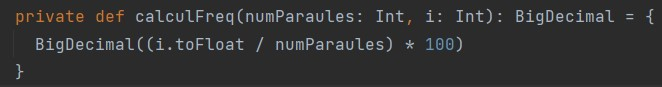
\includegraphics[height=2cm]{captures/primeraPart/ordreSuperior/toFloat.jpg}
				\end{center}
				
			\item \textbf{foldLeft}: Mètode que agafa una funció d'ordre superior i l'utilitzará per col·lapsar la col·lecció. Un exemple d'ús, per calcular la freqüència total de les paraules. Ens serveix per recorrer i guardar el valor anterior:
				\begin{center}
					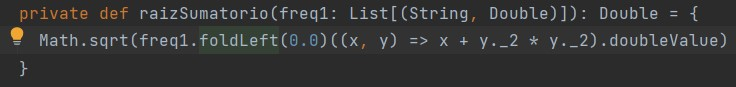
\includegraphics[height=1.8cm]{captures/primeraPart/ordreSuperior/foldLeft.jpg}
				\end{center}
				
			\item \textbf{map}: Mètode que aplica una funció a cada element de la col·lecció. L'hem utilitzat per calcular la freqüència normal. Exemple d'ús:
				\begin{center}
					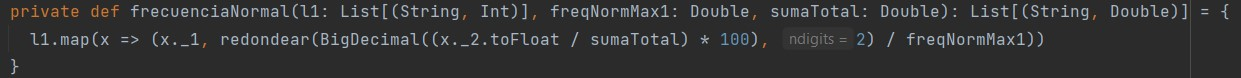
\includegraphics[height=1cm]{captures/primeraPart/ordreSuperior/map.jpg}
				\end{center}
				
			\item \textbf{setScale}: Mètode utilitzat per redondejar. Exemple d'ús:
				\begin{center}
					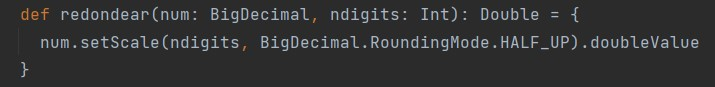
\includegraphics[height=1.5cm]{captures/primeraPart/ordreSuperior/setScale.jpg}
				\end{center}
				
			\item \textbf{compareTo}: Mètode comparar dues cadenes. L'utilitzem per saber quina de les dues cadenes hem d'avançar. Exemple d'ús:
				\begin{center}
					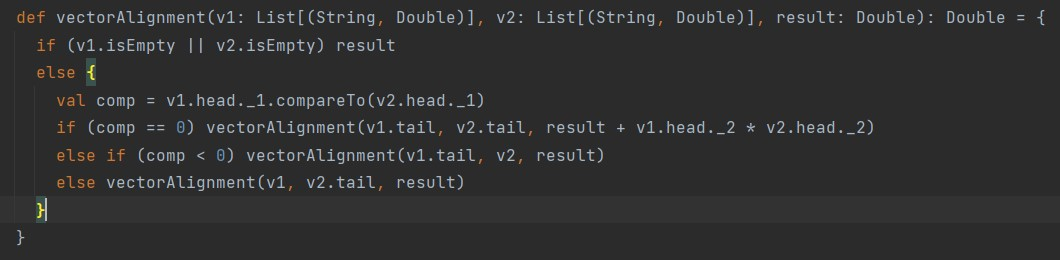
\includegraphics[height=3cm]{captures/primeraPart/ordreSuperior/compareTo.jpg}
				\end{center}
				
			\item \textbf{sliding}: Utilitzada per dividir la llista en n grames. Exemple d'ús:
				\begin{center}
					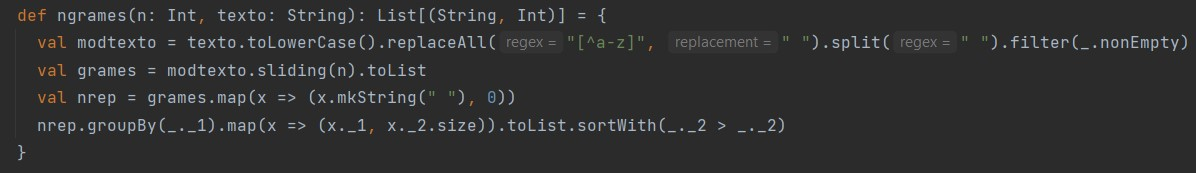
\includegraphics[height=2cm]{captures/primeraPart/ordreSuperior/sliding.jpg}
				\end{center}
				
			\item \textbf{groupBy}: Utilitza el predicat rebut per agrupar i formar un Map. L'utilizem agafant els nGrames (1 2) i formats com una cadena i els agrupem per key i així agrupem per nGrama. Exemple d'ús:
				\begin{center}
					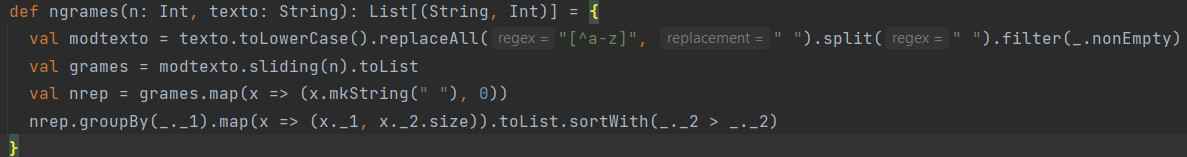
\includegraphics[height=2cm]{captures/primeraPart/ordreSuperior/groupBy.jpg}
				\end{center}
				
			\item \textbf{distinct}: Aquest mètode l'utilitzem per guardar només les paraules úniques, i així no repetir. Exemple d'ús:
				\begin{center}
					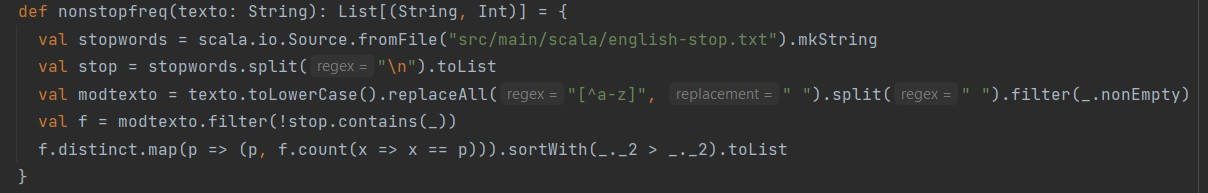
\includegraphics[height=2.5cm]{captures/primeraPart/ordreSuperior/distinct.jpg}
				\end{center}
		\end{itemize}
		
	\subsection{Segona Part}
		A la segona part no cal destacar cap funció d'ordre superior, totes les utilitzades són molt comunes.
		
		\subsubsection{Modificació MapReduce}

			\begin{itemize}
				\item S'han afegit dos paràmetres nous \textbf{numappers} i \textbf{numreducers}.
				\item A la línia 73 s'assigna numappers a nmappers.
				\item A la línia 108 s'assigna la longitud de l'entrada a mappersPendents.
				\item A la línia 125 s'assigna numreducers a nreducers.
			\end{itemize}

% Secció: Càlculs realitzats
\section{Càlculs realitzats}

	\begin{itemize}
		\item \textbf{input}:  List[(K1,List[V1])]
		\item \textbf{mapping}: (K1,List[V1]) => List[(K2,V2)]
		\item \textbf{reducing}: (K2,List[V2])=> (K2,V3)
		
		\begin{itemize}
		
			\item \textbf{mappingLlegir i reduccingLlegir}:
			Aquestes dos funcions ens permeten obtenir a partir del nom del fitxer que li passem com a V1, per obtenir la seva informació i així guardar-la en el objecte que s'ha creat com a diccionari InfoFicheros, més endavant. Això ens permet no tornar a cridar la funció parseViquipediaFile cada vegada que necessitem alguna informació d’algun fitxer. Per tant, en el mapping retornarem com a key el títol, y el valor una tupla de listes de la informació que té aquell fitxer.
			\begin{itemize}
				\item \textbf{K1}: Int, id que no necessitarem.
				\item \textbf{V1}: String, del nom del fitxer.
				\item \textbf{K2}: String, nom del fitxer
				\item \textbf{V2}: Tupla, de lista de Strings, amb cada una de la informació del fitxer.
				\item \textbf{V3}: Lista de tuplas de lista de Strings. Retornem el mateix que ha rebut, però la segona posició de la tupla, serà una List, ja que després ens serà més fàcil de treballar, en cas que li tinguem que enviar al MapReduce.
			\end{itemize}
			
			\item \textbf{mappingRef i reduccingRef}:
Aquestes funcions ens permetran calcular el nombre de vegades que surt una referencia entre tots els documents. Per això, retornem com a key 2, el nom de referencia i un comptador per després en el reduccing sumar-lo.
			\begin{itemize}
				\item \textbf{K1}: String, títol del document. No el farem servir ja que ens interessa només les referencies que té.
				\item \textbf{V1}: String, nom de la referencia, que utilitzarem com a K2.
				\item \textbf{K2}: String, es el nom de la referencia, ja que ens interessa agrupar per nom de la referencia.
				\item \textbf{V2}: Int, serà un 1, perquè es com un contador que després sumarem tots en el reduccing i així saber cuantes vegades surt.
				\item \textbf{V3}: Int, la suma de cuantes vegades ha sortit la refencia K2.
			\end{itemize}
			
			\item \textbf{mappingCombNoRef i reduccingCombNoRef}:´
Aquestes funcions son importants, perquè ens permeten combinar els documents sense repetirse entre ells i sense referenciar-se mútuament.
Per fer el mapping, li passem el títol amb el seu contingut. Però el que ens interessa es el títol, perquè a partir del diccionari, concretament la variable InfoFicheros.fitxTratar, que tenim ordenat prèviament, podem saber en quina posició està. Volem saber la posició que està ja que, ens permet agafar del InfoFicheros.fitxTratar, a partir d’aquella posició i ens permet no repetir amb els anteriors de la llista. Això ens permet tindre millor rendiment i eficiència. 
Dins d’aquest mètode recorrem la llsita sobrant de InfoFicheros.fitxTratar, i comprovem que no sigui el mateix nom, ja que no ens interessa i que no tingui una referencia d’aquell fitxer, ja que així no ens interessaria guardar-lo.
			\begin{itemize}
				\item \textbf{K1}: String, títol amb el que combinarem.
				\item \textbf{V1}: String, paraules del que no es rellevant.
				\item \textbf{K2}: String, títol serà el mateix que el K1, en cas de que es pugui combinar sinó serà  un espai en blanc. El espai en blanc el borrarem quan s’hagi acabat tot el MapReduce.
				\item \textbf{V2}: String, títol en cas de que es pugui combinar, sinó estarà buit.
				\item \textbf{V3}: List[String], que conté totes les combinacions possibles amb K2.
			\end{itemize}
			
			\item \textbf{mappingWC i reduccingWC}:
			Aquestes funcions ens permetran contar les ocurrències de cada paraula en cada fitxer. Es important que guardem com a K2, una tupla de títol i paraula, per agrupar-les. El value serà un comptador. Tindrà la mateixa idea que nombre de referencies.
			\begin{itemize}
				\item \textbf{K1}: String,  títol del document.
				\item \textbf{V1}: String, paraula que conté el document.
				\item \textbf{K2}: Tupla, de títol i paraula.
				\item \textbf{V2}: Int, comptador que utilitzarem per sumar.
				\item \textbf{V3}: Int, suma de valors que apareix aquella paraula en el document.
			\end{itemize}
			
			\item \textbf{mappingTF i reduccingTF}:
Aquesta funció és va pensar per reestructurar les ocurrències de les paraules, és a dir, ara tenim un Map amb una tupla com a Key i la ocurrència com a valor. Aleshores, aquestes dos funcions ens permetran tindre com a key, el títol del document, i com a value  una llista de tuples de paraula i ocurrència que te aquest document.
			\begin{itemize}
				\item \textbf{K1}: Tupla, títol i paraula.
				\item \textbf{V1}: Int, Ocurrencia que surt aquesta paraula en aquest títol, K1.
				\item \textbf{K2}: String, títol del document, per així poder agrupar en paraules i ocurrències.
				\item \textbf{V2}: Tupla, amb la paraula i la ocurrència.
				\item \textbf{V3}: Tupla, amb la paraula i la ocurrència.
			\end{itemize}
			
			\item \textbf{mappingTfIdf i reduccingTfIdf}:
Aquestes dos funcions ens permetrà calcular el tfidf. Per això ens interessa agrupar per paraules, i que el reduccing  rebi la paraula i una llista dels documents a on surt amb la seva ocurrència. Així, ja sabrem a quants documents surt aquella paraula.
			\begin{itemize}
				\item \textbf{K1}: String, títol del document.
				\item \textbf{V1}: Tupla, paraula i ocurrencia
				\item \textbf{K2}: String, paraula
				\item \textbf{V2}: Tupla, títol i ocurrencia
				\item \textbf{V3}: Tupla, títol i valor tfidf.
			\end{itemize}
			
			\item \textbf{mappingGirar i reduccingGirar}:
Aquestes dos funcions s’utilitzen per reestructurar la informació que ja tenim dels tfidf. Per tant convertirem de paraula (key), i tupla títol, tfidf a títol (key), paraula i tfidf. Això ens permet tindre una millor estructura per treballar més tard.
			\begin{itemize}
				\item \textbf{K1}: String, paraula dels diferents documents.
				\item \textbf{V1}: Tupla, títol i tfidf.
				\item \textbf{K2}: String, títol del document.
				\item \textbf{V2}: Tupla, paraula i tfidf.
				\item \textbf{V3}: Tupla, paraula i tfidf. Es important que ordenem ja que quan calculem el cosinesim, els tenim que tindre els elements.
			\end{itemize}
			
			\item \textbf{mappingRaizSumatorio i reduccingRaizSumatorio}:
Aquestes dues funcions, és van crear per calcular la part del denominador del càlcul del cosinesim de similitud, ja que, es fer la arrel del sumatori del mateix document. Aquest resultat el guardem al diccionari, per utilitzar-lo en el cosinesim.
			\begin{itemize}
				\item \textbf{K1}:  String, títol del document.
				\item \textbf{V1}: Tupla, paraula i tfidf.
				\item \textbf{K2}: String, títol del document
				\item \textbf{V2}:Double, valor del tfidf.
				\item \textbf{V3}: Double, resultat del càlcul del arrel del sumatori
			\end{itemize}
			
			\item \textbf{mappingCosinoSimil i reduccingCosinoSimil}:
En aquestes dues funcions els utilitzem per calcular el valor del cosinesim. El mapping rebrà el títol del document i la llista de documents amb el que pot combinar. Per tant, a partir d’aquí amb l’ajuda del diccionari agafarem la informació que necessitem per calcular-lo. 
			\begin{itemize}
				\item \textbf{K1}: String, títol del document
				\item \textbf{V1}: String, títol del document.
				\item \textbf{K2}: String, títol (K1) del document.
				\item \textbf{V2}: Tupla, títol del document combinat i el valor del cosinesim.
				\item \textbf{V3}: List[(String,Double)], títol del document combinat i el valor del cosinesim.
			\end{itemize}		
			
			\item \textbf{mappingFotos i reduccingFotos}:
			Aquestes dues funcions ens serveixen per a partir de totes les imatges que tenen els diferents documents, calcular el nombre mitjà de fotos.
			\begin{itemize}
				\item \textbf{K1}: String, titol del document.
				\item \textbf{V1}: String, nom de la foto.
				\item \textbf{K2}: Int, és una Key per poder-los agrupar i fer la suma després.
				\item \textbf{V2}: Int, quantitat de fotos que hi ha en un document.
				\item \textbf{V3}: Tupla, K2 i nombre mitjà.
			\end{itemize}
			
			\item \textbf{mappingNombrePromRef i reduccingNombrePromRef}:
			Aquestes dues funcions ens serveixen per a partir de totes les referències que tenen els diferents documents, calcular el nombre mitjà de referències.
			\begin{itemize}
				\item \textbf{K1}: String, titol del document.
				\item \textbf{V1}: String, referència.
				\item \textbf{K2}:  Int, és una Key per poder-los agrupar i fer la suma després.
				\item \textbf{V2}:  Int, quantitat de referències que hi ha en un document.
				\item \textbf{V3}:  Tupla, K2 i nombre mitjà.
			\end{itemize}
		\end{itemize}
	\end{itemize}

% Secció: Jocs de proves
\section{Jocs de proves}

	\subsection{Resultats Execucions Primera Part}
	
		\subsubsection{Freqüència de paraules}
		
			\begin{center}
				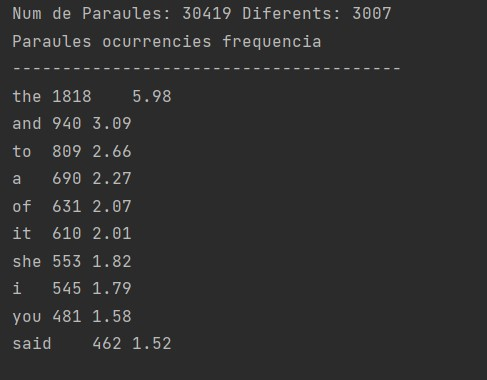
\includegraphics[height=7cm]{captures/primeraPart/freq/resultatFreq.jpg}
			\end{center}
		
		\subsubsection{Sense stop-words}
		
			\begin{center}
				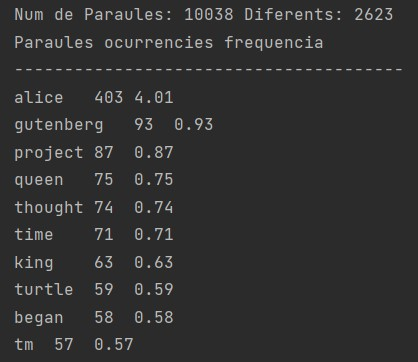
\includegraphics[height=8cm]{captures/primeraPart/sensestopwords/execucio.jpg}
			\end{center}
		
		\subsubsection{Distribució de paraules}
		
			\begin{center}
				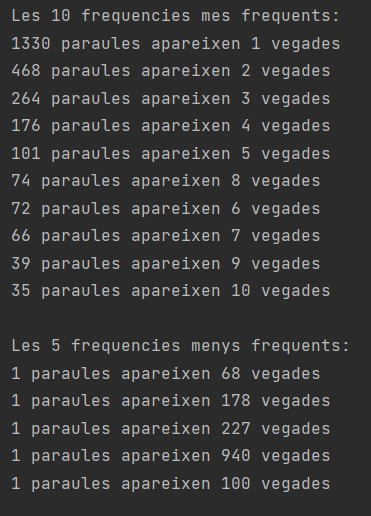
\includegraphics[height=8cm]{captures/primeraPart/distribucioParaules/execucio.jpg}
			\end{center}
		
		\subsubsection{Ngrames}
		
			\begin{center}
				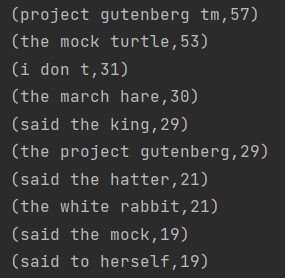
\includegraphics[height=7cm]{captures/primeraPart/ngrames/execucio.jpg}
			\end{center}
		
		\subsubsection{Vector space model}
		
			\begin{itemize}
			
				\item Resultat execució (\textbf{n = 0}):
			
				\begin{center}
					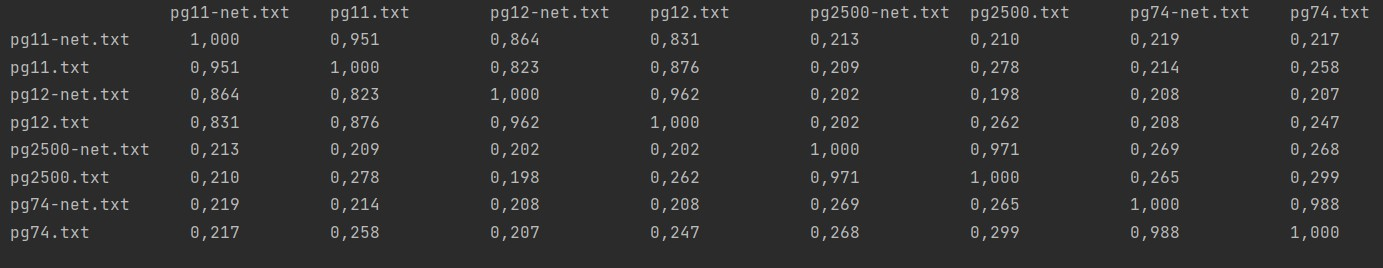
\includegraphics[height=3cm]{captures/primeraPart/vectorspacemodel/execucio0.jpg}
				\end{center}
				
				\item Resultat execució (\textbf{n = 2}):
				
				\begin{center}
					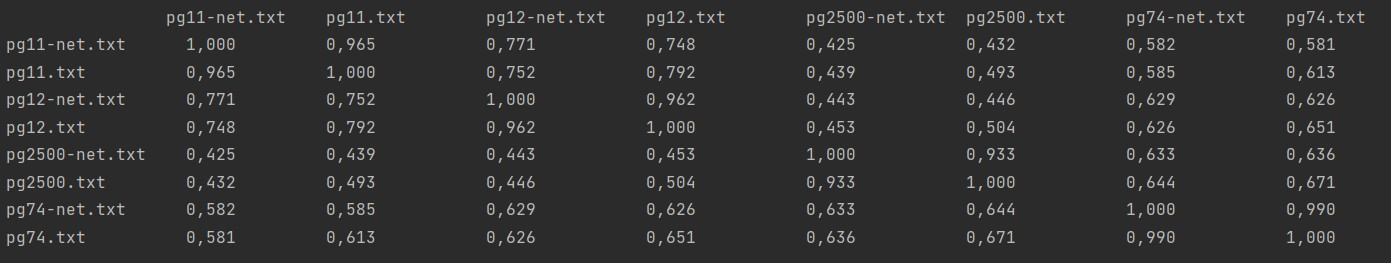
\includegraphics[height=3cm]{captures/primeraPart/vectorspacemodel/execucio2.jpg}
				\end{center}
				
				\item Resultat execució (\textbf{n = 3}):
				
				\begin{center}
					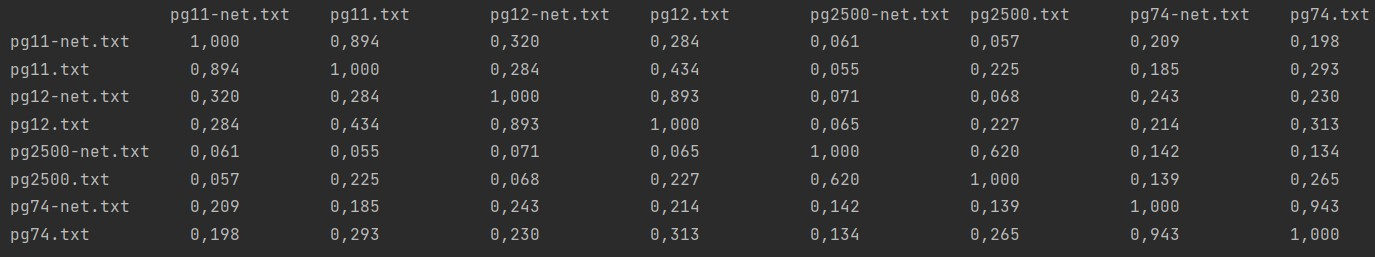
\includegraphics[height=1.5cm]{captures/primeraPart/vectorspacemodel/execucio3.jpg}
				\end{center}	
			
			\end{itemize}
			
	\subsection{Resultats Execucions Segona Part}
	
		\begin{itemize}
			\item numappers = 1, numreducers = 1 i 5000 fitxers:
			
				\begin{center}
					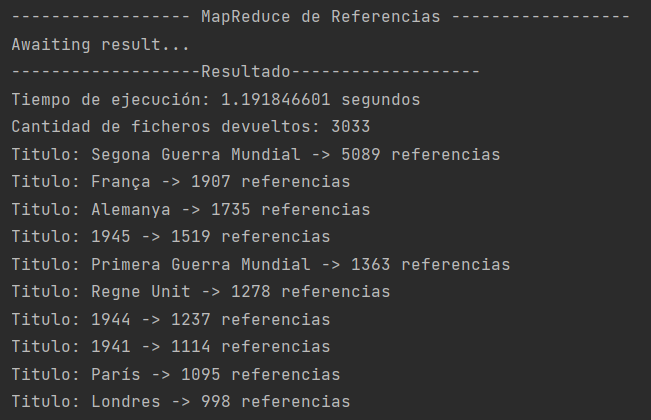
\includegraphics[height=5cm]{captures/segonaPart/joc1/1.png}
				\end{center}
				
				\begin{center}
					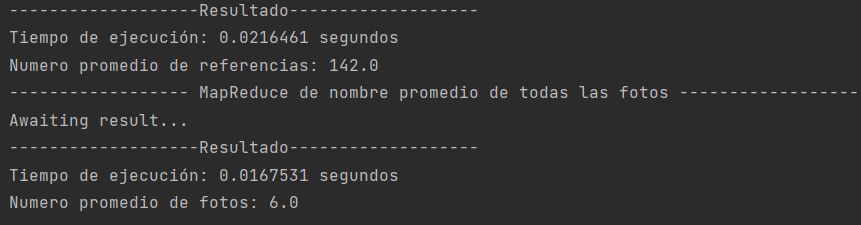
\includegraphics[height=3cm]{captures/segonaPart/joc1/2.png}
				\end{center}
				
				\begin{center}
					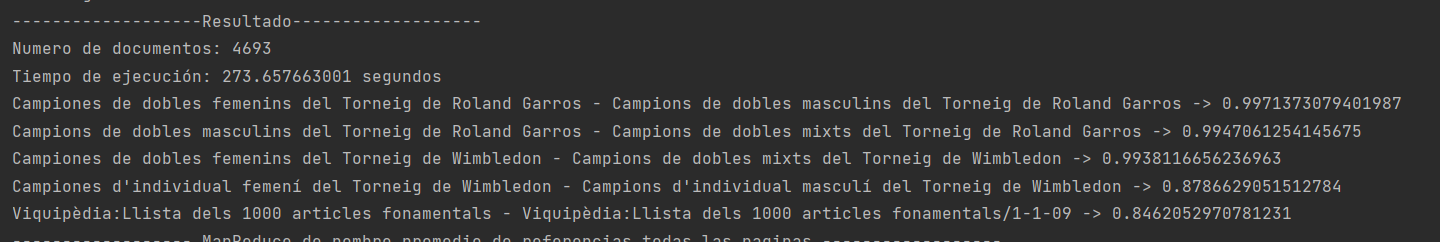
\includegraphics[height=1.5cm]{captures/segonaPart/joc1/3.png}
				\end{center}
				
				\begin{center}
					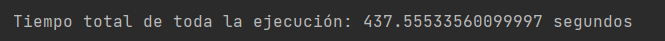
\includegraphics[height=1cm]{captures/segonaPart/joc1/4.png}
				\end{center}
			
			\item numappers = 20, numreducers = 12 i 5000 fitxers:
			
			\begin{center}
					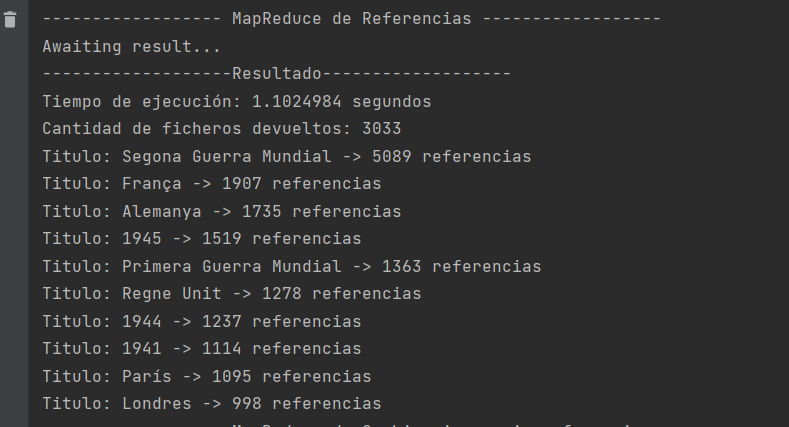
\includegraphics[height=5cm]{captures/segonaPart/joc2/1.png}
				\end{center}
				
				\begin{center}
					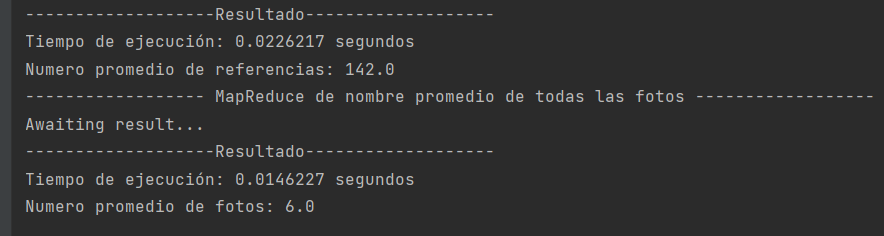
\includegraphics[height=3cm]{captures/segonaPart/joc2/2.png}
				\end{center}
				
				\begin{center}
					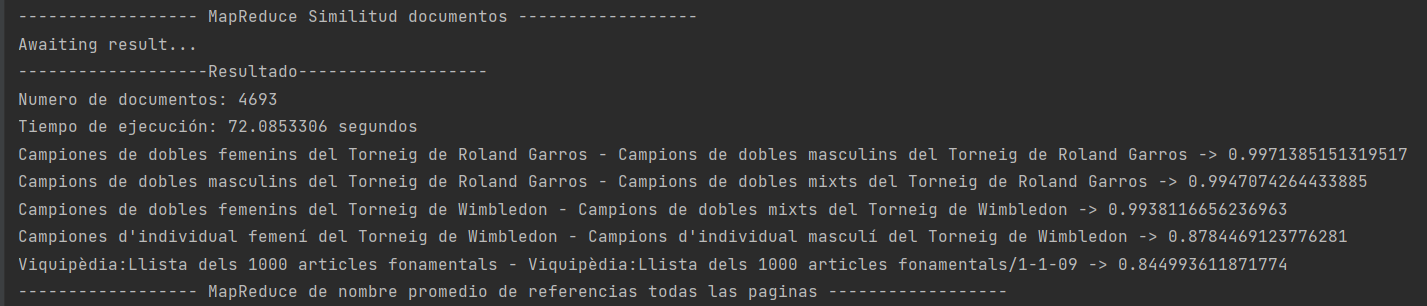
\includegraphics[height=2cm]{captures/segonaPart/joc2/3.png}
				\end{center}
				
				\begin{center}
					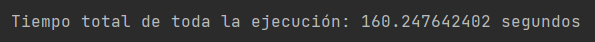
\includegraphics[height=1cm]{captures/segonaPart/joc2/4.png}
				\end{center}
				
				\item numappers = 12, numreducers = 8 i 1000 fitxers:
			
				\begin{center}
					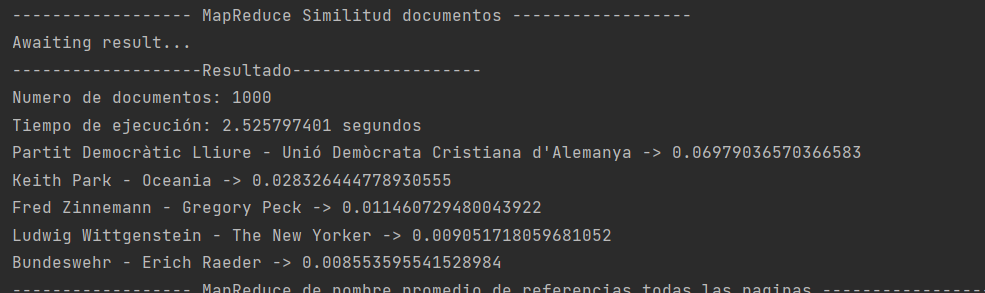
\includegraphics[height=3cm]{captures/segonaPart/joc3/1.png}
				\end{center}
				
				\begin{center}
					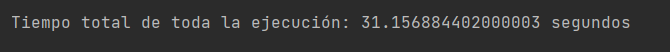
\includegraphics[height=1cm]{captures/segonaPart/joc3/2.png}
				\end{center}
				
				
		\end{itemize}


% Secció: Taula de rendiment
\section{Taula de rendiment}

	Per la realització de les diferents proves, s'ha utilitzat l'equip amb les següents especificacions.

	\subsection{Especificacions}
		
		\begin{center}
			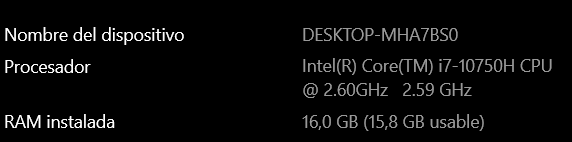
\includegraphics[height=4cm]{captures/especificacionsEquip/especificacions1.png}
		\end{center}
		
		\begin{center}
			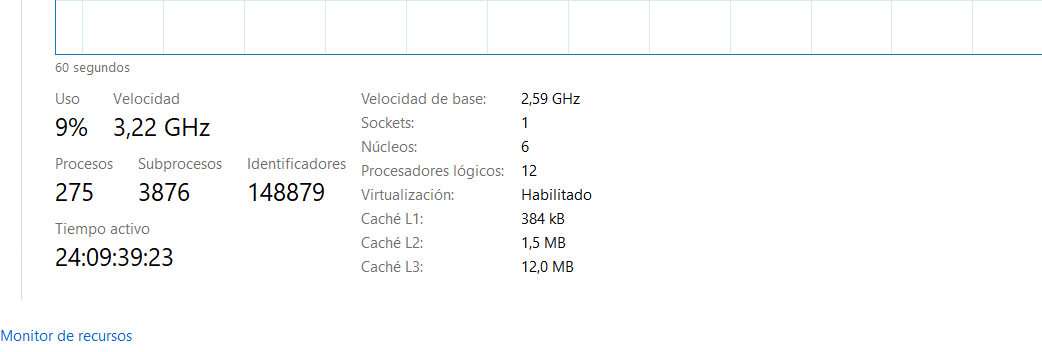
\includegraphics[height=5cm]{captures/especificacionsEquip/especificacions2.png}
		\end{center}
		
	\subsection{Taula dels actors}
	
		Les proves s'han realitzat amb tots els fitxers disponibles, i la taula representa per cada número d'actors, quants segons triga.
	
		\begin{table}[h!]
			\centering
			\begin{tabular}{||c c c c||} 
			 \hline
			 \multicolumn{4}{|c|}{Número d'actors} \\
			 \hline
			 1 & 4 & 10 & 20 \\ [0.5ex] 
			 \hline
			  437.55 & 173.42 & 133.28 & 160.24 \\ [1ex] 
			 \hline
			\end{tabular}
		\end{table}

% Secció: Altres consideracions
\section{Alltres consideracions}

Com s'indiquen a les proves anteriors, s'han realitzat amb tots els fitxers disponibles i s'ha aconseguit un molt bon temps. Per tant, molt contents amb el resultat final.


\end{document}


